\documentclass[10pt,a4paper]{beamer}

\usepackage{xcolor}
\usepackage{graphicx}
\usepackage{float}
\usepackage{listings}
\usepackage{enumerate}
\usepackage{pgfpages}
\usepackage{amsmath}
\usepackage{mathtools}
\usepackage{tensor}
\setbeameroption{show notes}
\setbeameroption{show notes on second screen=right}

\usetheme{Madrid}
\author{Kevin Maguire}
\defbeamertemplate*{footline}{shadow theme}
{\leavevmode
 \hbox{\begin{beamercolorbox}[wd=.5\paperwidth,ht=2.5ex,dp=1.125ex,leftskip=.3cm plus1fil,rightskip=.3cm]{author in head/foot}
\usebeamerfont{author in head/foot}\insertframenumber\,/\,\inserttotalframenumber\hfill\insertshortauthor
\end{beamercolorbox}
\begin{beamercolorbox}[wd=.5\paperwidth,ht=2.5ex,dp=1.125ex,leftskip=.3cm,rightskip=.3cm plus1fil]{title in head/foot}
    \usebeamerfont{title in head/foot}\insertshorttitle
\end{beamercolorbox}}
  \vskip0pt
}

\usetheme{Madrid}
\author{Kevin Maguire}
\title{Singular Lorentz Transformations and Pure Radiation Fields}
\date{\today}
\pagenumbering{arabic}

\begin{document}

\setbeamercovered{transparent}

\begin{frame}
\maketitle
\end{frame}

%LAYOUT

\begin{frame}
\frametitle{Layout}
\begin{enumerate}
\item<1->{Introduction: Lorentz Transformations}
\item<2->{Strange Minkowskian Line Element}
\item<3->{Singular Lorentz transformation}
\item<4->{$SL(2,\mathbb{C})$ Matrices of the Lorentz Transformation}
\item<5->{The Fractional Linear Transformation}
\item<6->{Infinitesimal Lorentz Transformation}
\item<7->{Pure Radiation conditions}
\end{enumerate}
\end{frame}

%INTRODUCTION

\begin{frame}
\begin{minipage}{6cm}
\frametitle{Introduction: Lorentz Transformations}
\begin{itemize}
\item<1->{A Lorentz transformation is defined by the preservation of the quadratic form $${x'}^2 + {y'}^2 + {z'}^2 - {t'}^2 = x^2 + y^2 + z^2 - t^2,$$ in the transformation $(x,y,z,t) \rightarrow (x',y',z',t')$}
\item<2->{Take the \textcolor{red}{Proper Orthochronous Lorentz Transformations(POLTs)} which form the \textcolor{red}{restricted Lorentz group} $SO^{+}(1,3)$}
\item<3->{In general lorentz transformations have two invariant null directions}
\end{itemize}
\end{minipage}
\begin{minipage}{4.5cm}
\includegraphics<4->[scale=0.4]{../Tex/figs/1_1.jpg}
\end{minipage}
\note{
\begin{itemize}
\item<3->{--Proper is det 1 . preserves the orientation of spacial axes, preserves handedness}
\item<3->{--orthochronous means time is always positive and the direction of time is preserved}
\item<5->{--Think of the standard Lornetz transformation, always two null directions at $x \pm t$}
\end{itemize}
}
\end{frame}

\begin{frame}
\frametitle{Layout}
\begin{enumerate}
\item<1>{Introduction: Lorentz Transformations}
\item<1>{Strange Minkowskian Line Element}
\item<0>{Singular Lorentz transformation}
\item<0>{$SL(2,\mathbb{C})$ Matrices of the Lorentz Transformation}
\item<0>{The Fractional Linear Transformation}
\item<0>{Infinitesimal Lorentz Transformation}
\item<0>{Pure Radiation conditions}
\end{enumerate}
\note{
\begin{itemize}
\item{derive a strange minkowskian line element}
\item{making a complicated transformation that keeps a single null geodesic fixed look trivial}
\end{itemize}
}
\end{frame}

%STRANGE MINKOWSKIAN LINE ELEMENT

\begin{frame}
\frametitle{Strange Minkowskian Line Element}
\begin{itemize}
\item<1->{Start with the Schwarzschild solution $$\epsilon {\mathrm{d}s}^2 = {\left(1 - \frac{2m}{r}\right)}^{-1} {\mathrm{d}r}^{2} + r^2 ({\mathrm{d}\theta}^2 + {{\sin}^2 \theta}{\mathrm{d} \phi}^2) - \left(1 - \frac{2m}{r}\right) {\mathrm{d}t}^2.$$}
\item<2->{Make the Eddington-Finkelstein coordinate transformation [2] $$u = t-r - 2m \ln(r-2m).$$}
\item<3->{Make further coordinate transformations to obtain $$\epsilon {\mathrm{d}s}^2 = \frac{r^2}{\cosh^{2}{\mu \xi}} ({\mathrm{d}\xi}^2 + {\mathrm{d}\eta}^2) - 2 {\mathrm{d}u}{\mathrm{d}r} - \left( \mu^{2} - \frac{2k}{r} \right) {\mathrm{d}u}^2.$$}
\item<4->{Taking the limit as the energy, $\mu \rightarrow 0$ gives The \textcolor{red}{Kasner Solution} $$\epsilon {\mathrm{d}s}^2 = r^2 ({\mathrm{d}\xi}^2 + {\mathrm{d}\eta}^2) - 2 {\mathrm{d}u}{\mathrm{d}r} - \frac{2k}{r} {\mathrm{d}u}^2.$$}
\end{itemize}
\note{
\begin{itemize}
\item<2->{First we are going to derive a strange form of the Minkowskian line element.. of the vacuum field equations, which will be familiar to most of us}
\item<3->{to remove the coordinate singularity in the Schwarzchild solution}
\item<4->{These transformations put the line element in a form where we can take the limit as the energy goes to 0}
\item<5->{It is easily shown with further coord transforms that this is Kasner, but it wont be done here}
\end{itemize}
}
\end{frame}

\begin{frame}
\frametitle{Strange Minkowskian Line Element}
\begin{itemize}
\item<1->{Then with $m = 0$ the strange Minkowskian line element is obtained $$\epsilon {\mathrm{d}s}^2 = r^2 ({\mathrm{d}\xi}^2 + {\mathrm{d}\eta}^2) - 2 {\mathrm{d}u}{\mathrm{d}r}.$$}
\item<2->{It is easily shown that $r = 0$ gives $$\epsilon {\mathrm{d}s}^2 = 0,$$ and thus is a null geodesic.}
\end{itemize}
\note{
\begin{itemize}
\item<2->{Its easily shown with suitable coordinate transforms that this is minkowskian line element}
\item<3->{This is best shown by calculating the geodesic equations after the Eddington-Finkelstein coord transforms, all zero if $u$ is proper time along the geodesic}
\end{itemize}
}
\end{frame}

\begin{frame}
\frametitle{Layout}
\begin{enumerate}
\item<1>{Introduction: Lorentz Transformations}
\item<1>{Strange Minkowskian Line Element}
\item<1>{Singular Lorentz transformation}
\item<0>{$SL(2,\mathbb{C})$ Matrices of the Lorentz Transformation}
\item<0>{The Fractional Linear Transformation}
\item<0>{Infinitesimal Lorentz Transformation}
\item<0>{Pure Radiation conditions}
\end{enumerate}
\note{LTs that leave one null invariant direction are constructed}
\end{frame}

%SINGULAR LORENTZ TRANSFORMATION

\begin{frame}
\frametitle{Singular Lorentz Transformation}
\begin{itemize}
\item<1->{Define an arbitrary complex parameter $\zeta \vcentcolon= \xi + i \eta ,$ to get the new line element[3] $$\epsilon {ds^2} = r^2 {d\zeta}{d\bar{\zeta}} - 2 {du}{dr}.$$}
\item<2->{The transformation $\zeta \rightarrow \zeta + w$, where $w \in \mathbb{C}$ is then trivial and leaves the single null geodesic $r = 0$ invariant.}
\item<3->{In Cartesian coordinates this transformation becomes

\begin{align}\nonumber
x' + i y' & = x + iy + w(t-z), \\\nonumber
z' - t' & = -r = z - t, \\\nonumber
z' + t' & = z+t + w(x - i y) + w(x + iy) + w\bar{w} (t-z).
\end{align}
}
\item<4->{Addition of complex numbers is commutative, and $w$ has two parameters, so \textcolor{red}{the singular Lorentz transformations form a 2-parameter abelian subgroup of the Lorentz group}}

\end{itemize}


\note{
\begin{itemize}
\item<3->{This is what we want, An LT which leaves one null invariant.}
\item<3->{The use in the previous coord transforms was to make this transformation look trivial}
\item<4->{So this is what the seemingly trivial transformation looks like in cartesians}
\item<4->{Again its clear that $r = 0$ keeps one direction fixed, as then z=t}
\item<5->{but it doesn't work both ways, not all 2 parameter abelian subgroups are singular lorentz transformations}
\end{itemize}
}
\end{frame}

\begin{frame}
\frametitle{Layout}
\begin{enumerate}
\item<1->{Introduction: Lorentz Transformations}
\item<1>{Strange Minkowskian Line Element}
\item<1>{Singular Lorentz transformation}
\item<1>{$SL(2,\mathbb{C})$ Matrices of the Lorentz Transformation}
\item<0>{The Fractional Linear Transformation}
\item<0>{Infinitesimal Lorentz Transformation}
\item<0>{Pure Radiation conditions}
\end{enumerate}
\note{
\begin{itemize}
\item{shown here that there is a 2 to 1 correspondence between SL(2,C) and POLTs}
\end{itemize}
}
\end{frame}

%SPECIAL LINEAR MATRICES OF THE LORENTZ TRANSFORMATION

\begin{frame}
\frametitle{$SL(2,\mathbb{C})$ Matrices of the POLT}
\begin{itemize}
\item<1->{There is a one to one correspondence between points in Minkowskian space-time and Hermitian matrices} 
\item<2->{Contruct the following matrix 
\begin{equation*}
A = 
\left( 
\begin{array}{cc}
t-z    & x + i y \\
x - iy & t+z \\
\end{array} 
\right),
\end{equation*}}
\item<3->{This is useful as its determinant is the Lorentz quadratic form modulo a sign $$\det(A(\vec{x})) = t^2 - x^2 - y^2 - z^2.$$}
\item<4->{Construct the transformation $A(\vec{x}') = U A(\vec{x}) U^{\dagger},$ where 
\begin{equation*} 
U = \left( 
\begin{array}{cc}
\alpha & \beta \\
\gamma & \delta \\
\end{array}
\right),
\end{equation*}

\noindent is an element of $SL(2,\mathbb{C})$}
\end{itemize}

\note{
\begin{itemize}
\item<2->{Complex Hermitian matrices have 4 independant components, so the element of such a matrix can be used to represent points in Minkowskian space-time.}
\item<5->{where $\alpha,\beta,\gamma,\delta$ are complex its an element of the special linear group. This means it has determinant 1. **write it on  the board** }
\end{itemize}
}
\end{frame}

\begin{frame}
\frametitle{$SL(2,\mathbb{C})$ Matrices of the POLT}
\begin{itemize}
\item<1->{$A(\vec{x}')$ and $A(\vec{x})$ have the same determinant so the above transformation preserves the Lorentz quadratic form, thus is is a Lorentz transformation.}
\item<2->{Write this transformation component wise

\begin{gather*} 
\left(
\begin{array}{cc}
t' - z' & x' + i y' \\
x' - i y' & t' + z' \\
\end{array}
\right)
=
\left(
\begin{array}{cc}
\alpha & \beta \\
\gamma & \delta \\
\end{array}
\right)
\left(
\begin{array}{cc}
t-z & x + i y \\
x - i y & t + z   \\
\end{array}
\right)
\left(
\begin{array}{cc}
\bar{\alpha} & \bar{\gamma} \\
\bar{\beta} & \bar{\delta} \\
\end{array}
\right), \\
 = \left(
\begin{array}{cc}
\alpha & \beta \\
\gamma & \delta \\
\end{array}
\right)
\left(
\begin{array}{cc}
(t-z)\bar{\alpha} + (x + iy)\bar{\beta} & (t-z)\bar{\gamma} + (x + iy)\bar{\delta} \\
(x - iy)\bar{\alpha} + (t+z)\bar{\beta} & (x-iy)\bar{\gamma} + (t+z)\bar{\delta} \\
\end{array}
\right).
\end{gather*}

}

\item<3->{Thus the \textcolor{red}{general relations}

\begin{gather*}
t' - z'  = (t-z)\alpha\bar{\alpha} + (x + iy)\alpha\bar{\beta} + (x - iy)\beta\bar{\alpha} + (t+z)\beta\bar{\beta},
\\
x' + iy'  = (t-z)\alpha\bar{\gamma} + (x + iy)\alpha\bar{\delta} + (x-iy)\beta\bar{\gamma} + (t+z)\beta\bar{\delta},
\\
t' + z'  = (t-z)\gamma\bar{\gamma} + (x + iy)\gamma\bar{\delta} + (x-iy)\delta\bar{\gamma} + (t+z)\delta\bar{\delta}.
\end{gather*}
}
\end{itemize}


\note{
\begin{itemize}
\item<2->{This is becasue the determinant of U is 1}
\item<3->{I want to show you an example calcualtion of U, to do this we write in component form}
\end{itemize}
}
\end{frame}

\begin{frame}
\frametitle{Example: Singular Lorentz transformation}
\begin{itemize}
\item<1->{Take the singular Lorentz transformation from earlier
\begin{align*}
t'-z' & = t-z, \\
x'+iy' & = x + iy + w(t-z), \\
t'+z' & = t+z + w(x-iy) + \bar{w} (x + iy) + w \bar{w} (t-z).
\end{align*}
}
\item<2->{Equate coefficients on the RHS of this equation with the RHS of the general relations on the previous slide to obtain

\begin{align*}
\alpha = \pm 1, \qquad & \beta = 0, \\
\gamma = \bar{w}\alpha, \qquad &  \delta = \alpha.
\end{align*}
}
\item<3->{So there are always \textcolor{red}{two} possible choices of U
\begin{equation*}
U = \pm
\left(
\begin{array}{cc}
1       & 0 \\
\bar{w} & 1 \\
\end{array}
\right)
\end{equation*}
}
\item<4->{Thus \textcolor{red}{there is a 2 to 1 correspondence between elements of $SL(2,\mathbb{C})$ and POLTs}}
\end{itemize}

\note{
\begin{itemize}
\item<3->{Where we have also used $det(U) = 1$}
\item<3->{becasue the sign doesn't matter is still a solution Eqn(27)}
\item<5->{A,A' are points in Minkowskian space time, and $\pm U$ are POLTs}
\end{itemize}
}
\end{frame}

\begin{frame}
\frametitle{Layout}
\begin{enumerate}
\item<1>{Introduction: Lorentz Transformations}
\item<1>{Strange Minkowskian Line Element}
\item<1>{Singular Lorentz transformation}
\item<1>{$SL(2,\mathbb{C})$ Matrices of the Lorentz Transformation}
\item<1>{The Fractional Linear Transformation}
\item<0>{Infinitesimal Lorentz Transformation}
\item<0>{Pure Radiation conditions}
\end{enumerate}
\note{
\begin{itemize}
\item{Connect Minkoswkian space to the 2-sphere by stereographic projection, so we can use points on a 2 sphere to think about LTs}
\end{itemize}
}
\end{frame}

%THE FRACTIONAL LINEAR TRANSFORMATION

\begin{frame}
\frametitle{Fractional Linear Transformation: Stereographic Projection}
\begin{itemize}
\item<1->{Use \textcolor{red}{Stereographic Projection} to map $\mathbb{S}^2$ to the \textcolor{red}{extended complex plane}, $\hat{\mathbb{C}} = \mathbb{C} \cup \{ \infty \}$

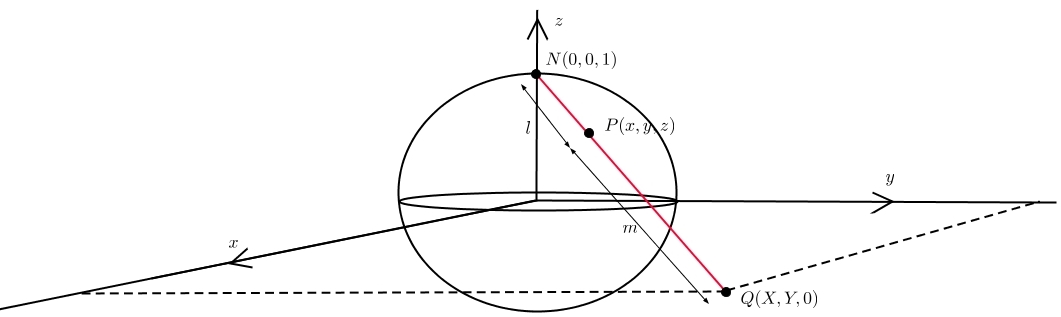
\includegraphics[scale=0.35]{../Tex/figs/4_1.jpg}
}
\item<3->{The algebraic relation for a unit vector is
\begin{equation*}
(x, y, z) = \begin{Huge} \left( \frac{\bar{\zeta} + \zeta}{\bar{\zeta}\zeta + 1}  ,i\frac{\bar{\zeta} - \zeta}{\bar{\zeta}\zeta + 1}, \frac{\bar{\zeta}\zeta - 1}{\bar{\zeta}\zeta + 1}  \right),
\end{Huge}
\end{equation*}
}
\item<4->{There is a one to one correspondence between $\mathbb{S}^2$ and $\hat{\mathbb{C}}$}
\end{itemize}

\note{
\begin{itemize}
\item<3->{As we know, stereographic projection doesn't map the point N at the top of the circle, so thats why we map N to infinity and need to consider the extended complex plane}
\item<3->{It can also be written in terms of $\theta$ and $\phi$}
\end{itemize}
}
\end{frame}

\begin{frame}
\frametitle{Fractional Linear Transformation: Stereographic Projection}
\begin{itemize}
\item<1->{Extend this to Minkowskian space-time[1]
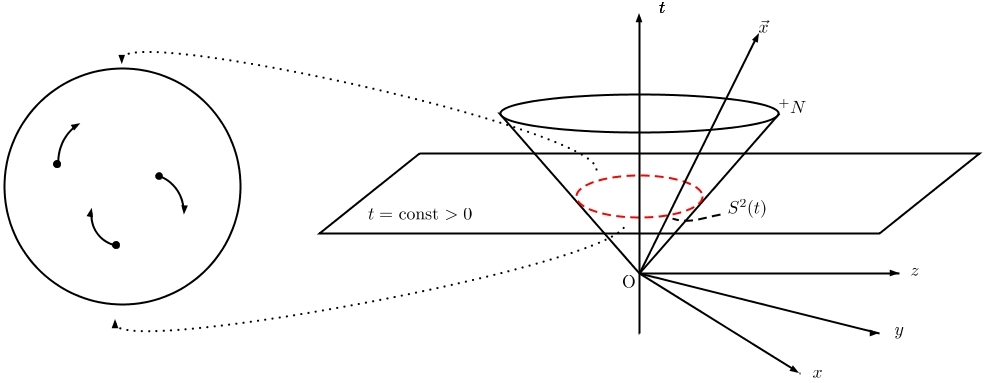
\includegraphics[scale=0.40]{../Tex/figs/4_5_2.jpg}
}
\item<2->{$(x, y, z ,t)$ $\leftrightarrow$ $\mathbb{S}^2$ $\leftrightarrow$ $\hat{\mathbb{C}}$}
\item<3->{So points in Minkowskian space-time can be written in the form
\begin{equation*}
\vec{x} = t
\begin{Huge}
\left( \frac{\bar{\zeta} + \zeta}{\bar{\zeta}\zeta + 1}  ,i\frac{\bar{\zeta} - \zeta}{\bar{\zeta}\zeta + 1}, \frac{\bar{\zeta}\zeta - 1}{\bar{\zeta}\zeta + 1},1  \right).
\end{Huge}
\end{equation*}
}
\end{itemize}

\note{
\begin{itemize}
\item<1->{all the points on the 2 sphere are generators of the future null cone in Minkowskian space time}
\item<1->{Can denote an LT by moving three arbitrary points along the surface of the sphere as the generators have dimension two, so to match the dim of the LT (it's 6) we need three of them}
\item<4->{Extra coord is becasue we take time into account now, now $\zeta$ has two parameters so x is in terms of two parameters, t just defines the direction}
\end{itemize}
}
\end{frame}

\begin{frame}
\frametitle{Fractional Linear Transformation}
\begin{itemize}
\item<1->{Make the transformation $\zeta \rightarrow \zeta'$ by constructing the matrix $A(\vec{x})$ and determining the matrix $U$.
\begin{equation*}
A(\vec{x}) = 
\left(
\begin{array}{ccc}
\frac{2t}{\zeta\bar{\zeta}+1} & & \frac{2t\zeta}{\zeta\bar{\zeta}+1} \\
 & & \\
\frac{2t\bar{\zeta}}{\zeta\bar{\zeta}+1} & & \frac{2t\zeta\bar{\zeta}}{\zeta\bar{\zeta}+1} \\
\end{array}
\right)
=
c_0\left(
\begin{array}{cc}
1           & \zeta \\ 
\bar{\zeta} & \bar{\zeta}\zeta \\ 
\end{array}
\right),
\end{equation*}
}
\item[]<2->{
\begin{equation*}
{c_0}'\left(
\begin{array}{cc}
1           & \zeta' \\ 
\bar{\zeta'} & \bar{\zeta'}\zeta' \\ 
\end{array}
\right)
=
\left(
\begin{array}{cc}
\alpha & \beta \\
\gamma & \delta \\
\end{array}
\right)
{c_0}\left(
\begin{array}{cc}
1           & \zeta \\ 
\bar{\zeta} & \bar{\zeta}\zeta \\ 
\end{array}
\right)
\left(
\begin{array}{cc}
\bar{\alpha} & \bar{\beta} \\
\bar{\gamma} & \bar{\delta} \\
\end{array}
\right).
\end{equation*}
}
\item<3->{Solve for $\zeta'$ to get the \textcolor{red}{fractional linear transformation}
\begin{equation*}
\zeta' = \frac{(\bar{\gamma} + \bar{\delta}\zeta)}{(\bar{\alpha} + \bar{\beta}\zeta)},
\end{equation*}
}
\item<4->{There is a \textcolor{red}{one to one correspondence between POLTs and fractional linear transformations}}
\end{itemize}

\note{
\begin{itemize}
\item<2->{These are null directions}
\item<2->{Refer to eqn (27) which should be on the board}
\item<3->{AS we did in the previous example, determine $U$}
\item<5->{Remember we had $\pm U$ now the signs will cancel in the denominator and numerator}
\end{itemize}
}
\end{frame}

\begin{frame}
\frametitle{Layout}
\begin{enumerate}
\item<1>{Introduction: Lorentz Transformations}
\item<1>{Strange Minkowskian Line Element}
\item<1>{Singular Lorentz transformation}
\item<1>{$SL(2,\mathbb{C})$ Matrices of the Lorentz Transformation}
\item<1>{The Fractional Linear Transformation}
\item<1>{Infinitesimal Lorentz Transformation}
\item<0>{Pure Radiation conditions}
\end{enumerate}
\note{
\begin{itemize}
\item{temp}
\end{itemize}
}
\end{frame}

%INFINITESIMAL LORENTZ TRANSFORMATION

\begin{frame}
\frametitle{Infinitesimal Lorentz Transformation}
\begin{itemize}
\item[]<1->{
\begin{equation*}
U = \pm
\left(
\begin{array}{cc}
1 + \epsilon a & \epsilon b \\
\epsilon c & 1 + \epsilon f \\
\end{array}
\right),
\end{equation*}}
\item[]<2->{$$\bar{x}^i = x^i + \epsilon \tensor{L}{^{i}_{j}} x^j + O(\epsilon^2),$$
where 
\begin{equation*}
\tensor{L}{^i_j} = 
\left(
\begin{array}{cccc}
0            & -2a_2        & (b_1 - c_1) & (b_1+c_1)\\
2a_2         & 0            & (b_2+c_2)   & (b_2 - c_2) \\
-(b_1 - c_1) & -(b_2 + c_2) & 0           & -2a_1 \\
(b_1 + c_1)  & (b_2-c_2)    & -2a_1       & 0 \\
\end{array}
\right)
\end{equation*}}
\item[]<3->{
\begin{equation*}
\frac{d^2 x^i}{ds^2} = \tensor{L}{^{i}_{j}}(s) \frac{d x^j}{ds}.
\end{equation*}}
\end{itemize}

\note{
\begin{itemize}
\item<2->{This was done in a recent lecture(Relativistic QM) so I wont do it}
\item<2->{Where a,b,c,d are complex}
\item<4->{Take many infinitesimal LT steps along a particles trajectory and let $\epsilon$ go to zero}
\end{itemize}
}
\end{frame}

\begin{frame}
\frametitle{Infinitesimal Lorentz Transformation: Lorentz Force}
\begin{itemize}
\item<1->{Can rewrite this equation in terms of the particles $3$-velocity $\vec{u}$, in component form
\begin{align*}
\frac{d}{dt} (\gamma(u) u^{(1)}) & = -2a_2u^{(2)} + (b_1 - c_1)u^{(3)} + b_1 + c_1, \\ 
\frac{d}{dt} (\gamma(u) u^{(2)}) & = 2a_2 u^{(1)} + (b_2 + c_2) u^{(3)} + b_2 - c_2,\\ 
\frac{d}{dt} (\gamma(u) u^{(3)}) & = -(b_1 - c_1) u^{(1)} - (b_2 + c_2 )u^{(2)} - 2a_1,\\ 
\frac{d\gamma(u)}{dt} & = (b_1 + c_1)u^{(1)} + (b_2 - c_2) u^{(2)} - 2a_1 u^{(3)}.
\end{align*}}
\item<2->{Define the $3$-vectors
\begin{align*}
\vec{P} & = (b_1+c_1,b_2-c_2,-2a_1), \\
\vec{Q} & = (b_2 + c_2, -(b_1 - c_1),-2a_2).
\end{align*}}

\end{itemize}

\note{
\begin{itemize}
\item<1->{temp}
\end{itemize}
}
\end{frame}

\begin{frame}
\frametitle{Infinitesimal Lorentz Transformation: Lorentz Force}
\begin{itemize}
\item<1->{Writing the equations in terms of these 
\begin{equation*}
\frac{d}{dt} (\gamma(u)\vec{u}) = \vec{P} + \vec{u} \times \vec{Q},
\end{equation*}}
\item<2->{This is the same form as the \textcolor{red}{Lorentz force}}
\item<3->{Make the Identification
\begin{equation}
\vec{P} = \frac{q}{m} \vec{E}, \qquad \vec{Q} = \frac{q}{m}\vec{B},
\end{equation}}
\item<3->{\textcolor{red}{To be compatible with special relativity the Lorentz force must depend on $\vec{u}$ in this way}. So the Lorentz force is a special case of a charged particle moving along a world line in minkowskian space-time generated by an infinitesimal Lorentz transformation.}
\end{itemize}

\note{
\begin{itemize}
\item<1->{temp}
\end{itemize}
}
\end{frame}

\begin{frame}
\frametitle{Layout}
\begin{enumerate}
\item<1>{Introduction: Lorentz Transformations}
\item<1>{Strange Minkowskian Line Element}
\item<1>{Singular Lorentz transformation}
\item<1>{$SL(2,\mathbb{C})$ Matrices of the Lorentz Transformation}
\item<1>{The Fractional Linear Transformation}
\item<1>{Infinitesimal Lorentz Transformation}
\item<1>{Pure Radiation conditions}
\end{enumerate}
\note{
\begin{itemize}
\item{temp}
\end{itemize}
}
\end{frame}

%PURE RADIATION CONDITIONS

\begin{frame}
\frametitle{Pure Radiation Conditions}
\begin{itemize}
\item<1->{The fractional linear transformation of the infinitesimal transformation is
\begin{equation*}
\zeta' = \frac{\zeta + \epsilon(\bar{c} - \bar{a}\zeta) + O(\epsilon^2)}{1 + \epsilon(\bar{a} + \bar{b} \zeta) + O(\epsilon^2)}.
\end{equation*}}
\item<2->{Fixed points of the system are given by $\zeta = \zeta'$ and correspond to null directions}
\item<3->{With this condition solve the fractional linear transformation for $\zeta$ $$\bar{\beta}\zeta^2 + (\bar{\alpha}- \bar{\delta})\zeta - \bar{\gamma} = 0.$$}
\item<4->{A quadratic means it has \textcolor{red}{two roots in general}}
\item<5->{Interested in the singular root case so take the descriminant equal to zero to get
\begin{equation*}
a^2 +bc = 0.
\end{equation*}
\noindent refer to this as the \textcolor{red}{quadratic condition}.}
\end{itemize}

\note{
\begin{itemize}
\item<5->{This is one of the things I said I would show earlier}
\item<6->{THIS WILL BE VERY IMPORTANT, **write on the board**}
\end{itemize}
}
\end{frame}

\begin{frame} 
\frametitle{Pure Radiation Conditions}
\begin{itemize}
\item<1->{The $a$ and $b$ are related to $\vec{E}$ and $\vec{B}$ through the Lorentz force as
\begin{eqnarray*}
a_1 = -\frac{1}{2} E^3, \qquad b_2 = \frac{1}{2}(E^2 + B^1), \qquad c_1 = \frac{1}{2} (E^1 + B^2),\\
a_2 = -\frac{1}{2} B^3, \qquad b_1 = \frac{1}{2} (E^1 - B^2), \qquad c_2  = \frac{1}{2} (B^1 - E^2). 
\end{eqnarray*}}
\item<2->{Then the real and imaginary parts of the quadratic condition give us the relations
\begin{gather*}
{|\vec{E}|}^2 = {|\vec{B}|}^2, \\
\vec{E} \cdot \vec{B} = 0.
\end{gather*}}
\item<3->{These are the familiar pure radiation conditions. Thus \textcolor{red}{if the world line of a charged particle is generated by an infinitesimal Lorentz transformation then the particle is moving in a pure radiation EM field.}}
\end{itemize}

\note{
\begin{itemize}
\item<2->{q/m factors suppresed for convenience}
\end{itemize}
}
\end{frame}

\begin{frame}
\frametitle{Layout}
add in the contents

\note{
\begin{itemize}
\item{MAny other things can be shown, I will finally show one small lemma of this result}
\end{itemize}
}
\end{frame}

%ITS LONG ENOUGH ALREADY
%PROPAGATION DIRECTION OF EM RADIATION
%
%\begin{frame} 
%\frametitle{Propagation direction of EM Radiation}
%\begin{itemize}
%\item<1->{temp}
%\end{itemize}
%
%\note{
%\begin{itemize}
%\item<1->{temp}
%\end{itemize}
%}
%\end{frame}

%%%%%%%%%%%%%%%%%%%%%%%%%%%%%%%%%%%%%%%%%%%%%%%%%%%%%%%%%%%%%
%FRAME TEMPLATE
%\begin{frame} 
%\frametitle{temp}
%\begin{itemize}
%\item<1->{temp}
%\end{itemize}
%
%\note{
%\begin{itemize}
%\item<1->{temp}
%\end{itemize}
%}
%\end{frame}

\begin{frame}
\frametitle{References}
\begin{itemize}
\item[1]{ J.L. Synge - ``Relativity: The Special Theory'' - North Holland Publishing Company (1965)}
\item[2]{ D. Finkelstein - ``Past-Future Asymmetry of the Gravitational Field of a Point Particle'' - Phys.Rev.Vol 110, (1958) - \url{http://journals.aps.org/pr/pdf/10.1103/PhysRev.110.965}}
\item[3]{ P.A. Hogan, C.Barrab\`es - ``Advanced General Relativity: Gravity Waves, Spinning Particles and Black Holes'' - Oxford University Press (May 2013)}
\item[4]{ I. Robinson ``Spherical Gravitational Waves'' - Phys.Rev.Lett. 4 (1960) 431-432 - \url{http://journals.aps.org/prl/pdf/10.1103/PhysRevLett.4.431}}
\item[5]{ P.A Hogan, C. Barrab\`es - ``Singular Null Hypersurfaces'' - World Scientific Pub Co Inc (April 2004)}
\item[6]{ R. Penrose, W. Rindler - ``Spinors and Space-Time: Volume 1, Two-Spinor Calculus and Relativistic Fields'' - Cambridge University Press, (Feb 1987)}
\item[7]{ Tristan Needham - ``Visual Complex Analysis'' - Clarendon Press, Oxford (1997)}
\item[8]{ Various Authors - ``Space-Time and Geometry: The Alfred Schild Lectures'' - University of Texas Press (March 21, 2012)}
\end{itemize}
\end{frame}

\end{document}
